\documentclass[12pt]{exam}

\RequirePackage{GE05}
% this inputs graphicx, too
\RequirePackage{comment}
\RequirePackage[hypertex]{hyperref}
    \hypersetup{colorlinks=true,urlcolor=blue,linkcolor=red}

\def\ClassName{The Global Economy}
\def\Category{Professor David Backus}
\def\HeadName{Group Project \#1}
\newcommand{\phm}{\phantom{--}}
\newcommand{\NX}{\mbox{\it NX\/}}

%\noprintanswers 
\printanswers 

\begin{document}
\parindent = 0.0in
\parskip = \bigskipamount
\thispagestyle{empty}%
\Head

\centerline{\large \bf \HeadName: Macroeconomic Data} 
\centerline{Revised:  \today}

\medskip
{\it Submit via Blackboard by 9am February 2.}

\begin{questions}
\question {\it National Accounts in Beerblastia.} 
Several years ago,
a group of entrepreneurial Stern graduates pooled their resources and
purchased an island in the Caribbean that they named Beerblastia.
After a few years of rapid growth, Beerblastia's economy has begun
to stagnate.  On the principle that there's no good policy without
good data, the head of the government has asked you to serve as
the country's first Chief National Accountant and compile a
set of aggregate statistics for last year.

On your first day on the job, you receive reports 
from the following local producers:  
%
\begin{itemize}
\item Local coffee shops sold \$16,000 % ??was 15k 
worth of coffee to local consumers. 
Their expenses were:  
purchases of coffee from local growers (\$3,000), 
wages and fringe benefits (\$9,000), % ?? was 8k 
and rent (\$4,000).

\item Coffee growers sold coffee beans to 
coffee shops (the \$3,000 noted above) and Starbucks* (\$5,000).
(Asterisks denote foreign companies.) 
Expenses include labor (\$4,000) and land rental (\$4,000).

\item Local fruit producers harvested and sold 
\$50,000 worth of bananas: 
60\% to domestic consumers, 20\% to Chiquita*, 
and the remainder to a local subsidiary of Dole*. 
Labor costs were \$30,000.  
They also spent \$20,000 on new banana-picking machinery
produced by a French* company.  

\item The Dole subsidiary produced \$20,000
worth of canned bananas, all of which were sold to domestic
consumers. Dole paid \$5,000 in wages to locals and repatriated
the remaining income to its foreign owners.  

\item The government raised \$2,000 from Beerblastians in taxes, 
paid government administrators \$2,000, 
and paid \$1,000 in pensions to retired Beerblastians.  

\item Two Beerblastians got short
consulting jobs in the US that paid them \$500 each.
\end{itemize}
%
Your mission:  take these reports and construct national accounts.  
Your accounts should include 
\begin{parts}
\part measures of value added producers in Beerblastia (10~points); 
\part GDP (5~points);
\part measures of the expenditure components (consumption,
investment, government purchases of goods and services, and net
exports) (10~points); 
\part show how saving and investment are related (10~points); 
and 
\part measures of the government's revenues, expenses, 
and surplus or deficit (5~points).  
\end{parts} 

\begin{solution}
The core of the answer is these numbers 
(all expressed in thousands):  
%
\begin{center}
\tabcolsep = 0.15in
\begin{tabular}{lcccccc} 
\hline\hline%
       &&  \multicolumn{4}{c}{Final Sales} \\ 
\cline{3-6}
Producer   &  Value Added &  $C$ & $I$ & $G$ & $\NX$      \\
\hline\hline%
Coffee shops &  13  & 16  \\
Coffee growers & 8 & & & & 5 \\
Fruit producers & 50 & 30 & 20 & & 10--20 \\
Dole Sub  & 10 & 20  \\
Govt production & 2 \\
\hline 
Total & 83 & 66 & 20 & 2 & --5 \\
\hline\hline%
\end{tabular}
\end{center}

\begin{parts} 
\part Value added for each producer is sales revenue minus 
intermediate inputs.  
In some cases, we can connect that to payments to labor
and capital, but it's not necessary.  
Note that value added is not the same as final sales: 
sales at the last stage of the value chain.
Thus, for example, the Dole sub has final sales of 20k, 
but since the fruit input costs 10k, value added is only 10k.  
Note that we have ignored the consultants:  they're potentially 
a source of local income, but the production is done outside 
the country and doesn't appear in local value-added or GDP.  

\part Each final sale is allocated in the table 
to the appropriate expenditure category.  
GDP is the sum of value added by all (local) producers, 
and also the sum of the expenditure components (final sales).  

\part Given the expenditure components, 
we compute (gross domestic) saving as 
\[
    S \;=\; Y - C - G \;=\; 83 - 66 - 2 = 15 .
\]

\part $S$ computed above equals $ I + \NX$.  As it must!  
One way to think about this:  investment of 20 
is financed by saving (15) and foreign capital ($\NX = -5$
corresponds to a purchase of 5 of local assets
by people in other countries).  

\part Revenues are 2k, expenses are 3k, so the surplus is $ -1$k 
(a deficit).  
Note that pensions are an expense of the government, 
even though they are not a purchase of a good or service 
and do not contribute (directly) to GDP.  
%\end{comment}
\end{parts} 
\end{solution} 
%\end{questions}
%\end{document} 


% --------------------------------------------------------------------

\question {\it Prices and quantities in Darkenbourg.}  
Earlier this month, the
Kingdom of Darkenbourg applied for admission to the European
Union. The ultra-efficient ``Eurocrats'' at the European Commission
returned the application in just three days, arguing that crucial
aggregate statistics were missing. The government has hired you as
a consultant to rectify the omissions. Reviewing the application,
you discover that it reported only GDP at current prices (ie,
nominal GDP) and did not report either real GDP or inflation.

You begin your contract by spending one day a week at the Royal
Office of Statistics teaching the staff about national accounting.
They tell you that Darkenbourg produces only three products, 
who quantities and prices are listed below:  
\begin{center}
\tabcolsep = 0.12in
\begin{tabular}{lcccccc}
\hline\hline%
     &\multicolumn{2}{c}{Food}
     &\multicolumn{2}{c}{Energy} 
     &\multicolumn{2}{c}{Computers}\\%
\cline{2-7}%
Year &   Quantity & Price   & Quantity &    Price   &  Quantity & Price    \\
\hline\hline%
1995 &     100    & 12 & 100 & 15 & 80  & 20  \\%
%\hline%
2005 &     90    & 18 & 100 & 15 & 160 & 10 \\%
\hline\hline%
\end{tabular}
\end{center}
Your job is to compute the following statistics from this data so
that Darkenbourg's application can be amended and resubmitted:
%
\begin{parts}
\part Nominal GDP, real GDP, and the price deflator for both
years. 
Use 1995 as the base year.  
(10~points)

\part A consumer price index for both years. 
As before, use 1995 as the base year.  (10~points)

\part The annualized rates of inflation over the period 1995-2005
based on the GDP deflator and the CPI, respectively.
Explain briefly why the two measures of inflation are different.  
(5~points)

\part Suppose rich and poor people consume similar baskets of goods,
with the exception that poor people do not buy computers.
Which group has the higher rate of inflation?  
(A qualitative answer is sufficient.) 
(5~points)
\end{parts}


\begin{solution}
The calculations are summarized by:
\begin{center}
\begin{tabular}{lcccc}
\hline\hline
         &  Nominal GDP  & Real GDP   &  GDP Deflator  & CPI \\
 \hline\hline
1995     &   4300     & 4300   &  1.000  &  4300  \\
2005     &   4720     & 578    &  0.817  &  4100 \\
Growth (\%)  & 9.8    &  34.4  &  --18.3 &  --4.6  \\
Annualized (\%) & 0.9 & 3.0    & --2.0   & --0.5 \\
\hline\hline
\end{tabular}
\end{center}

\begin{parts} 
\part 
Nominal GDP is the sum of the
product of current prices times current quantities; 
in 1995, for example, it equals 
$12\times 100+ 15 \times 100 + 20\times 80 = 4300 $. 
Real GDP here is the sum of 1995 prices times
current quantities; in 2005, for example, 
it equals 
$12\times 90 + 15 \times 100 + 20\times 160 = 5780$.  
(In the jargon of the professionals, 1995 is the base year.) 


\part The CPI is the sum of
current prices times (in this case) 1995 quantities; 
in 2005, it equals 
$18\times 100+ 15\times 100 + 10\times 80 = 4100$.

\part Growth rates are computed this way.  The total growth rate
between 1995 and 2005 is the ratio of the 2005 figure to the 1995
figure, minus one.  And if you want to make it a percentage, 
you multiply by 100.
Thus the growth rate $g$ of the CPI (the CPI-based inflation rate, in other words) is the solution to
\[
    1 + g \;=\; 4100/4300 \;=\; 0.9535 ,
\]
so that $g = - 4.65\%$.  
The annualized growth rate solves
\[
    (1 + g)^{10} \;=\; 4100/4300
\]
or
\[
    (1 + g) \;=\; (4100/4300)^{1/10}
\]
so that $g = -0.475\%$.  Growth rates for other variables are
computed the same way.
The numbers in the table have been rounded.  

Notice that this inflation is different from one computed
from the GDP deflator.
Why?  Roughly, because they weight goods differently.  
The details are a P2C2E. 

\part Here's another weighting example.  
Since the poor in this example don't buy computers, 
and computers have prices that are falling rapidly, 
their inflation rate will be higher than the inflation 
rate for rich people.  

As it turns out, the logic is right but the example
gives you the wrong idea.  Our best estimates are that the poor 
have had lower inflation rates in recent times than the rich.
Why?  Because the poor buy things at Wal-Mart, 
whose prices have stayed low, 
and the rich buy services, whose price has gone up.  
\end{parts} 
\end{solution}
%\end{questions}
%\end{document} 

% ----------------------------------------------------------------------
\question {\it Saving and investment in the US and China.}  
In recent years, China has run a substantial trade surplus 
(positive net exports) 
(over 5\% of GDP) and the US a similar deficit.  
The Chinese surplus has become a political issue in the US;
it implies that China is a net purchaser of foreign assets
and a net exporter of goods.    
Using ``Country Data'' from the Economist Intelligence Unit (EIU)
or another source, 
download the expenditure components of GDP (measured at current prices) 
for both countries for the period 1990-present.  Use them to
%
\begin{parts}
\part Graph saving, investment, and net exports as ratios to GDP.  
Define saving here as $S = Y - C - G $. 
(10~points) 

\part Document the similarities and differences between the two countries
with respect to saving, investment, and net exports.  
(10~points) 

\part 
Speculate freely about the factors that might have led to 
 differences in net exports between the two countries.  
(10~points) 
\end{parts}
%
If you have trouble accessing the relevant data, 
follow these steps:  
\begin{itemize}
\item Bobst Virtual Business Library $\Rightarrow$ 
Country Information $\Rightarrow$   \\
EIU Country Data  $\Rightarrow$ 
CountryData \\  
(If you are off-campus, 
you will be asked to provide your NYU id and password.) 
\item Once there, click on Data Selection to choose the countries, 
time period, and series of interest.  
\end{itemize} 

\begin{solution}

\begin{parts}
\part See the figures in today's slides.  
They're constructed so that net exports
is the difference between saving and investment.  

\part The most striking feature of the figures is that 
both saving and investment are substantially higher 
in China than the US.
Over the recent past, the saving rate has increased in China, 
and decreased in the US.
Since the trade balance (net exports) is the difference 
between saving and investment, 
the changes in saving rates have led to 
a trade surplus in China and deficit in the US.
Any discussion of the Chinese trade surplus, 
then, should also address the 
Chinese saving rate:  the two are intertwined.  

The question is why the saving and investment rates are so 
different.  
Ideas welcome.
One line of thought is that capital markets are poorly developed
in China, so people save a lot to insure themselves against
misfortune:  poor pensions, bank failure, inflation, 
health care costs, and so on.  
We often see that as countries develop, saving rates go down, 
so perhaps we'll see that in China over the next couple 
decades.  
  
\part  
Some see disaster, others see capital moving around the world
to the most profitable opportunities.
How would you argue for one or the other?  
Which do you think it is?  
\end{parts} 
%\end{solution}
%\end{questions}

%\begin{center}
%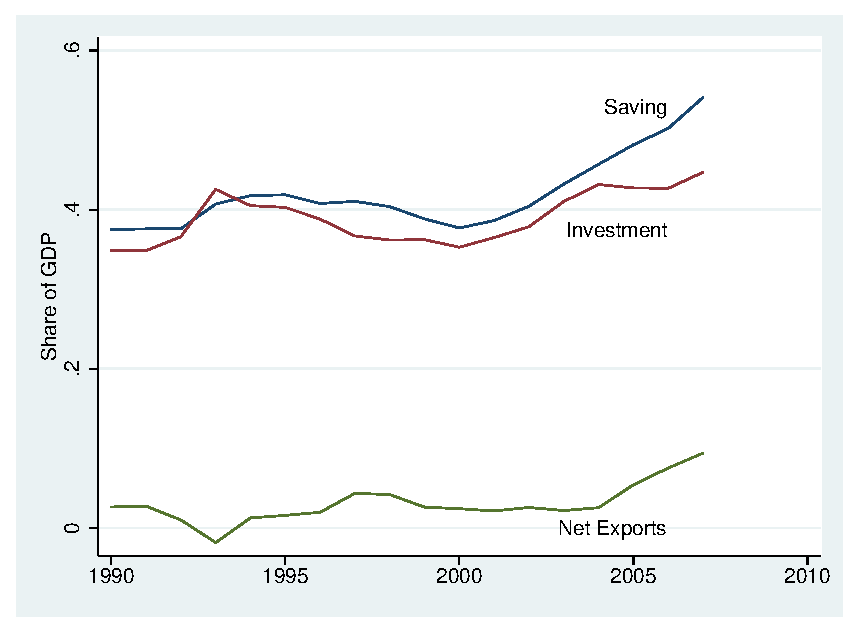
\includegraphics[scale=0.8]{shares_china.eps} \\
%\vspace*{0.2in} 
%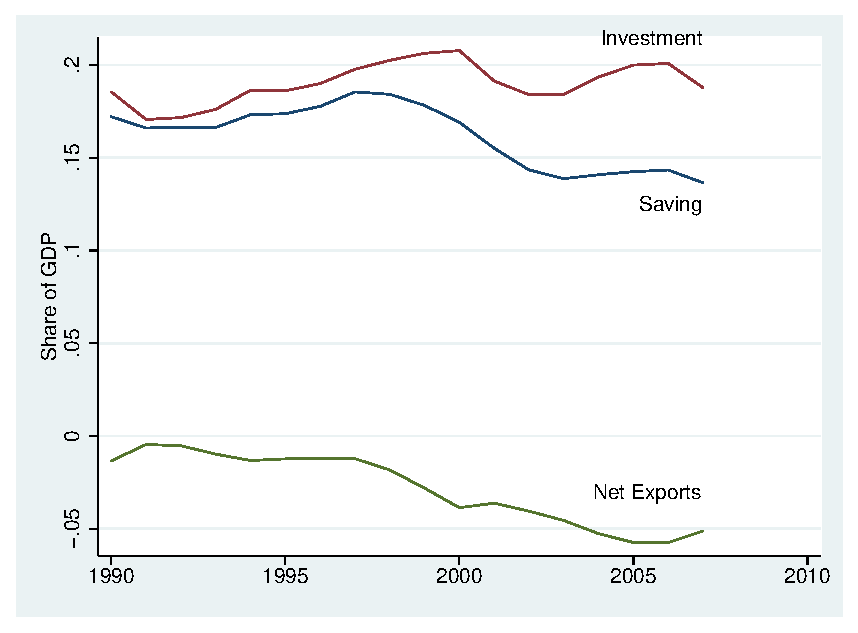
\includegraphics[scale=0.8]{shares_us.eps} 
%\end{center}

\end{solution}
\end{questions}


\vfill \centerline{\it \copyright \ \number\year \ 
NYU Stern School of Business}

\end{document} 

